\documentclass[
  11pt,
  singlespacing,
  liststotoc,
  toctotoc,
  headspline
]{fphw}

\usepackage{alphabeta}
\usepackage{lmodern}

\usepackage{fontenc}
\usepackage{xgreek}
\usepackage{xunicode}
\usepackage{xltxtra}

\usepackage[Greek,Latin]{ucharclasses}
\setTransitionsForGreek{\setlanguage{greek}}{\setlanguage{american}}

\setromanfont[Mapping=tex-text]{Linux Libertine}

\setmainfont{CMU Serif}
\setsansfont{CMU Sans Serif}
\newfontfamily{\greekfont}{CMU Serif}
\newfontfamily{\greekfontsf}{CMU Sans Serif}

\setmainfont{GFS Didot}

\usepackage[]{unicode-math}
\setmathfont{Latin Modern Math}

\usepackage[backend=bibtex,style=authoryear,natbib=true]{biblatex}

\usepackage{graphicx}
\usepackage{booktabs}
\usepackage{listings}
\usepackage{enumerate}
\usepackage{float}
\usepackage{minted}

\usepackage[hidelinks]{hyperref}

\title{Τελική Απαλλακτική Εργασία}
\author{Ιάκωβος Μαστρογιαννόπουλος - Κωνσταντίνος Καμαρόπουλος}
\institute{Πανεπιστημιο Δυτικης Αττικης \\ Τμημα Μηχανικων Πληροφορικης και Υπολογιστων}
\class{Διαχείριση Γνώσης}
\professor{Αθανάσιος Κιούρτης}

\begin{document}

\includegraphics[width=25mm]{Figures/Logo}
\maketitle

\begin{abstract}
  Αυτή είναι η τελική εργασία για το μάθημα <<Διαχείριση Γνώσης>> των φοιτητών:
  \begin{itemize}
      \item Ιάκωβος Μαστρογιαννόπουλος, 713242017102
      \item Κωνσταντίνος Καμαρόπουλος, 71346830
  \end{itemize}

  Η εργασία έχει ως βασικό σκοπό να γίνει κατανόηση του αντικειμένου της διαχείρισης γνώσης μέσω ενός παραδείγματος το οποίο επιλέχθηκε από την ομάδα. Η εργασία έχει δύο τμήματα, το πρώτο που είναι το πρακτικό κομμάτι για το πως μπορεί ένας αναλυτής να πάρει κάποια δεδομένα, να τα μετατρέψει σε πληροφορίες και γνώση. Το δεύτερο μέρος είναι πολύ πιο θεωρητικό και από την πλευρά ενός οργανισμού ο οποίος δέχεται την γνώση και προσπαθεί να την επεξεργαστεί για να την μεταφέρει και παρακάτω, με την χρήση του μοντέλου του Kotter. Τα προγράμματα έχουν αναπτυχθεί στην γλώσσα προγραμματισμού Python, έκδοσης 3.9 και έχει φτιαχτεί ενά Dockerfile που σημαίνει ότι μπορεί να τρέξει σε οποιοδήποτε λειτουργικό σύστημα που τρέχει Docker.
\end{abstract}

\newpage
\tableofcontents
\listoffigures
\listoftables

\newpage
\label{Chapter1}

\section{Διαδικασία ανακάλυψης γνώσης}

Στο πρώτο τμήμα της εργασίας, θα γίνει η ανάλυση του σεναρίου που επιλέχτηκε και θα παρουσιαστεί το πως πραγματοποιήθηκε η διαχείριση των δεδομένων για να βγει το συμπέρασμα και η γνώση στην τελική της μορφή.

\subsection{Επιλογή σεναρίου}

Σε όποιον αρέσει να ταξιδεύει στον κόσμο, κατά μεγάλη πιθανότητα θα έχει βρεθεί σε μία κατάσταση που δεν θα μπορεί να εύκολα να αποφύγει. Σε αρκετές χώρες, το νόμισμα το οποίο έχουν δεν είναι το νόμισμα της χωράς που κατοικεί και συνήθως αναγκάζετε ο ταξιδιώτης να ανταλλάξει τα χρήματα του στο τοπικό νόμισμα. Ένας τρόπος που μπορεί να αποφύγει, βέβαια το πρόβλημα είναι να χρησιμοποιεί μόνο την τραπεζική του κάρτα για όλες τις συναλλαγές, αλλά αυτό δεν είναι η λύση του προβλήματος, αλλά μόνο η αποφυγή του. Η λύση του προβλήματος αυτού ήταν και η δημιουργία του Ευρώ στα κράτη που ανήκουν Ευρωπαϊκή Ένωση (Ε.Ε.) και στην Ευρωζώνη. Έτσι, ένας Έλληνας μπορεί να ταξιδέψει σε μία χώρα που βρίσκετε μέσα στην Ε.Ε. και με το ίδιο νόμισμα να μπορεί να κάνει συναλλαγές εύκολα. Τι γίνετε όμως στις χώρες που δεν ανήκουν στην Ευρωζώνη; \par
Αρκετές χώρες έχουν λύση αυτό το πρόβλημα με την γραφείων των συναλλαγών (trade currency offices) που σκοπός τους είναι να πηγαίνει ο ταξιδιώτης και να μπορεί να ανταλλάξει το νόμισμα του στο τοπικό νόμισμα με κέρδος προς το γραφείο. Εκεί όμως ξεκινάει ένα άλλο πρόβλημα, που έχει \href{https://www.youtube.com/watch?v=6zwiArr3jYE}{\textbf{παρουσιαστεί πολλές φόρες σε βίντεο}}, το πρόβλημα της εκμετάλλευσης. Πολλά από αυτά τα γραφεία, βάζουν υπερβολικά μεγάλα ποσοστά και κρατάνε πολλή μεγάλο χρηματικό πόσο. Αυτό με κάποιον τρόπο θα πρέπει να βρεθεί μία λύση για να σταματήσει να υπάρχει αυτό το πρόβλημα.

\subsection{Επιλογή δεδομένων}

Τα δεδομένα τα οποία επιλέχτηκαν βρίσκονται σε ένα dataset το οποίο ήταν αποθηκευμένο σε CSV αρχείο, το οποίο \href{https://www.kaggle.com/dhruvildave/currency-exchange-rates}{\textbf{βρέθηκε στην ιστοσελίδα του Kaggle}}. Το συγκεκριμένο αρχείο τροποποιήθηκε κατάλληλα και κρατήθηκαν τα δεδομένα τα οποία ήταν χρήσιμα για την συγκεκριμένη περίπτωση. Τα δεδομένα αυτά ήταν το exchange rate του Ευρώ σε αλλά νομίσματα. \par
Χρησιμοποιήθηκε το Pandas module της Python για να διαβάσει τα δεδομένα και να μετατρέψει τις πληροφορίες που συγκεντρώθηκαν, μετατράπηκαν σε Dataframe και αποθηκεύτηκαν σε XML. Ο κώδικας είναι ο εξής:

\begin{minted}{py}
# Clean dataset implementation
def create_dataframe(path, dataset_path='./forex.csv') -> pd.DataFrame:
  # Read data from the CSV source file
  dataset = pd.read_csv(dataset_path)
  dataset.to_xml(path)

  # Keep only the info that is needed
  dataset = dataset.where(dataset['currency'] == 'EUR').dropna()
  dataset = dataset.where(dataset['high'] < 2).dropna()
  dataset = dataset.where(dataset['high'] > 0.2).dropna()

  # Dictionary
  clean_dataset = {
    'high': dataset['high'],
    'low': dataset['low'],
    'open': dataset['open'],
    'close': dataset['close']
  }

  # Parse dictionary to new DataFrame, save it and return this back
  clean_dataset = pd.DataFrame(clean_dataset)
  clean_dataset.to_csv('./dataset.csv')
  return clean_dataset
\end{minted}

\subsection{Εξόρυξη δεδομένων}

Υπάρχουν διάφοροι μέθοδοι που μπορούν να πραγματοποιηθεί εξόρυξη δεδομένων. Η μέθοδος που επιλέχτηκε για την συγκεκριμένη εργασία είναι η συσταδοποίηση (clustering). Ένας clustering αλγόριθμος χωρίζει το δείγμα που δέχεται σε μικρότερες ομάδες με ένα κοινό χαρακτηριστικό. Οι δύο clustering αλγόριθμοι που επιλέχτηκαν είναι ο KMeans και ο MeanShift.

\begin{figure}[H]
  \centering
  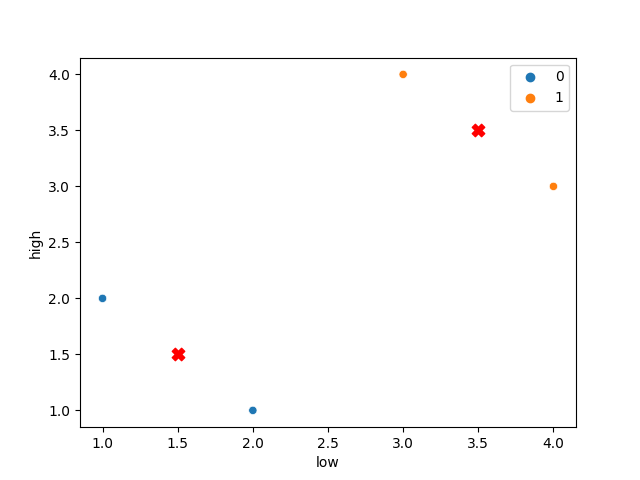
\includegraphics[width=100mm]{Figures/k_means_example.png}
  \caption{Παράδειγμα Clustering}
  \label{fig:example}
\end{figure}

\subsubsection{Υλοποίηση και αποτελέσματα KMeans}

Ο KMeans είναι ένας απλός clustering αλγόριθμος που βγάζει αρκετά πιστά δεδομένα.

\begin{minted}{py}
# KMeans implementation
def kmeans(
    dataframe: pd.DataFrame, n_clusters=4, path: str = "k_means_cluster.png"
  ) -> None:
  k_means = KMeans(n_clusters=n_clusters, init="k-means++", random_state=0)
            .fit(dataframe)

  sns.scatterplot(data=dataframe, x="low", y="high", hue=k_means.labels_)
  plt.scatter(
    k_means.cluster_centers_[:, 0], k_means.cluster_centers_[:, 1], marker='X',
    c="r", s=80, label="centroids"
  )
  plt.savefig(path)
  plt.show()
\end{minted}

\begin{figure}[H]
  \centering
  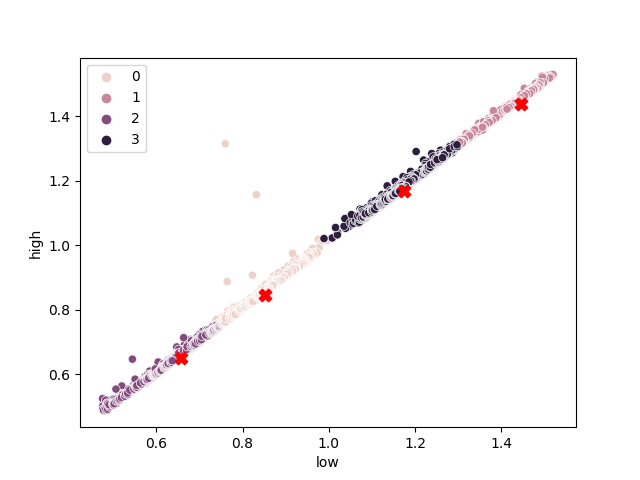
\includegraphics[width=100mm]{Figures/k_means_cluster.png}
  \caption{Αποτελέσματα KMeans}
  \label{fig:k_means}
\end{figure}

\subsubsection{Υλοποίηση και αποτελέσματα MeanShift}

Ο MeanShift είναι ένας εναλλακτικός clustering αλγόριθμος ο οποίος είναι λίγο πιο αργός αλλά τείνει στο να βγάζει πιο πιστά αποτελέσματα από ότι ο KMeans.

\begin{minted}{py}
# MeanShift implementation
def mean_shift(dataframe: pd.DataFrame) -> None:
  bandwidth = estimate_bandwidth(dataframe, quantile=0.1, n_samples=100)
  clusters = MeanShift(bandwidth=bandwidth, bin_seeding=True).fit(dataframe)

  sns.scatterplot(data=dataframe, x="low", y="high", hue=clusters.labels_)
  plt.scatter(
    clusters.cluster_centers_[:, 0], clusters.cluster_centers_[:, 1], marker='x', c="r",
    s=80, label="centroids"
  )
  plt.savefig('mean_shift_cluster.png')
  plt.show()
\end{minted}

\begin{figure}[H]
  \centering
  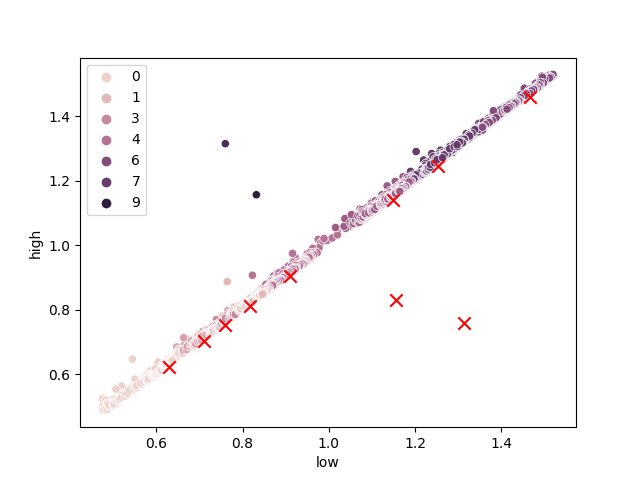
\includegraphics[width=100mm]{Figures/mean_shift_cluster.png}
  \caption{Αποτελέσματα MeanShift}
  \label{fig:mean_shift}
\end{figure}

\subsubsection{Σχολιασμός αποτελεσμάτων}
\label{chap:results}

Τα αποτελέσματα των δύο αλγορίθμων παρουσιάζονται στα Σχήματα~\ref{fig:k_means} και ~\ref{fig:mean_shift}. Παρότι οι δύο αλγόριθμοι είναι αρκετά διαφορετικοί μεταξύ τους, τα αποτελέσματα είναι σχεδόν ίδια. Ο KMeans έχει χωρίσει τα clusters σε 4, ενώ ο MeanShift σε 10. Σε ένα πιο πρακτικό σενάριο, μοιάζει ο KMeans να είναι πιο ελεγχόμενος, ένω ο MeanShift πιο πιστός στα πραγματικά δεδομένα. Για παράδειγμα, στον τομέα της Επεξεργασίας Εικόνας, ο KMeans θεωρείτε καλύτερος εφόσον παράγει παρόμοια αποτελέσματα αρκετά πιο γρήγορα από τον MeanShift.

\label{Chapter2}

\section{Θεωρητικό υπόβαθρο της διαχείρισης γνώσης}

\subsection{Διαχωρισμός δεδομένων, πληροφορίας και γνώσης}

\begin{problem}
  ``Δεδομένα: ουσιαστικοποιημένο ουδέτερο πληθυντικού της μετοχής δεδομένος, έχει δύο σημασίες:

  \begin{enumerate}
    \item στοιχεία, πληροφορίες, σε δυαδική μορφή που εισάγονται προς επεξεργασία σε έναν ηλεκτρονικό υπολογιστή ή προβάλλονται ως έξοδος σε μια περιφερειακή συσκευή
    \item στοιχεία, πληροφορίες, που έχουν λάβει δυαδική μορφή και έχουν αποθηκευτεί σε σκληρό δίσκο ή άλλο μέσο.
  \end{enumerate}

  Στην πληροφορική ότι αφορά το λογισμικό (όχι το υλισμικό) είναι δεδομένα. Ακόμη και τα προγράμματα που εκτελούνται εμπεριέχονται σε αρχεία, τα εκτελέσιμα αρχεία, που τα δεδομένα τους είναι εντολές για το τι πρέπει να κάνει το πρόγραμμα. Όταν ξεκινάει ο υπολογιστής φορτώνει από προκαθορισμένη θέση του σκληρού δίσκου τα δεδομένα που του λένε που θα βρει αποθηκευμένα τα εκτελέσιμα αρχεία του λειτουργικού συστήματος. Μετά το υλισμικό ότι υπάρχει είναι δεδομένα.''

  \href{https://el.wiktionary.org/wiki/%CE%B4%CE%B5%CE%B4%CE%BF%CE%BC%CE%AD%CE%BD%CE%B1}{\textbf{Ορισμός <<Δεδομένα>> στο Βικιλεξικό}}
\end{problem}

Τα δεδομένα τα οποία αρχικά είχαν συλλεχθεί ήταν τα exchange rates όλων των νομισμάτων σε άλλα νομίσματα.

\begin{problem}
  ``Πληροφορία: θηλυκό ουσιαστικό που στην θεωρία της πληροφορίας είναι η τυχαία τιμή ή ο συνδυασμός τιμών εντός της επιτρεπόμενης πληροφοριακής εντροπίας χωρίς αναγκαστικά να μεταφέρει σημασιολογικό κώδικα.''

  \href{https://el.wiktionary.org/wiki/%CF%80%CE%BB%CE%B7%CF%81%CE%BF%CF%86%CE%BF%CF%81%CE%AF%CE%B1}{\textbf{Ορισμός <<Πληροφορία>> στο Βικιλεξικό}}
\end{problem}

Πληροφορία είναι μία συλλογή δεδομένων που έχει επεξεργαστεί για να μπορεί να γίνει περισσότερη χρήση του και να βγει ένα αποτέλεσμα. Στο συγκεκριμένο παράδειγμα, κρατήθηκαν μόνο τα δεδομένα του Ευρώ και έτσι το νέο αρχείο ήταν συγκεντρωμένο με πιο καθαρές πληροφορίες σχετικές με το θέμα.

\begin{problem}
  ``Γνώση: θηλυκό ουσιαστικό που είναι οι πληροφορίες που αποκτά κάποιος και οι παραστάσεις που σχηματίζει για τον κόσμο και τα πράγματα μετά από την νοητική επεξεργασία των εμπειρικών δεδομένων''

  \href{https://el.wiktionary.org/wiki/%CE%B3%CE%BD%CF%8E%CF%83%CE%B7}{\textbf{Ορισμός <<Γνώση>> στο Βικιλεξικό}}
\end{problem}

Οι γνώσεις που μπορούν να θεωρηθούν από τα αποτελέσματα της εφαρμογής που μελετήθηκαν στο Κεφάλαιο~\ref{chap:results}. Με αυτά, μπορεί ο οποιοσδήποτε να παρατηρήσει ότι η διαφορά μεταξύ υψηλότερης και κατώτερης τιμής στα exchange offices παραμένουν παρόμοια κατά μέσο όρο στην πάροδο του χρόνου και μόνο σε συγκεκριμένες περιπτώσεις το θέμα γίνετε τραγικά κακό.

\subsection{Κύκλος ζωής διαχείρισης γνώσης}

\subsection{Μοντέλο αλλαγών του Kotter}


\appendix
\section{Βιβλιογραφία}
\label{AppendixA}

\begin{itemize}
  \item Διαφάνειες Διαχείρισης Γνώσης, Α. Κιούρτης, 2021
\end{itemize}
\end{document}